\documentclass{article}

\usepackage{amssymb}
\usepackage{amsmath}
\usepackage{listings}
\usepackage{amsmath}
\usepackage{float} 
\usepackage[a4paper]{geometry} 
\usepackage{graphicx}

\begin{document}
\title{Unit 26 | Mathematics for IT Practitioners \\ \vspace{1.5cm} Assignment 2 | Probability, Sequences, Number Systems and Statistics}
\author{Daniel Easteal}
\date{March 2017}
\maketitle
\newpage
\tableofcontents
\newpage
\section{Introduction}
In this assignment I will be going through the mathematics behind probability, sequences number systems and statistical analysis of data. 
\section{Series and Sequences and Probability}
\subsection{-3, 1, 5, 9, 13 \dots}
\subsubsection{nth term}
Find a formula for the nth term of this sequence and find the 17th term using your nth term formula. Also calculate the sum of the first 17 terms of this sequence.
\[
	-3, 1, 5, 9, 13, \dots
\]
To start off with I will need to find the difference between the numbers in the sequence that I have been given because I believe that this is a linear progression and this will get half the answer for me. Looking at the numbers, each number is 4 more than the previous one...
\[
	\overbrace{-3, 1}^{+4}	\quad	\overbrace{1, 5}^{+4}	\quad	\overbrace{5, 9}^{+4}	\quad	\overbrace{9, 13}^{+4}
\]
Now that I know the distance from each number to the next, I can then formulate the initial equation to be $$ n=4x+?$$ so now I just need to work out what the "?" will be. Now, for the first term the x value will be one and so we would have 4 as the value, but the first value is actually -3, so we will need to adjust to this and have the equation subtract 7 from all the values so now the equation will look like this:
\[
	n=4x-7
\]
We can then test this to ensure that it works by testing the 4th value as we know the answer to that:
\[
	4(4)-7	\Rightarrow 16-7	\Rightarrow 9
\]
And this answer lines up with the answer that we are given in the question so I know that the equation is correct.  
\[
	\therefore n^{th} term = 4x-7
\]
\subsubsection{17th term}
It is very simple to find the 17th term, or really any term of the sequence once you know the nth term formula, all that you have to do is replace the "x" with the term that you want and then you have to work the equation through. For this question it would go like this: 
\[
	4x-7 \Rightarrow 4(17)-7 \Rightarrow 68-7 \Rightarrow 61
\]
\[
	\therefore 17^{th} term = 61
\]
\subsubsection{Sum of terms}
To sum the sequence that we have been given we will have to use the sum of an arithmetic sequence progression equation and this looks like this: 
\[
	\frac{n(a_{1} + a_{n})}{2}
\]
this sequence sequence is an arithmetic sequence because it advances in the series by adding numbers rather than multiplying by them. In this equation, all of the symbols start for something and I will explain them below:
\begin{align}

	n &= \mbox{represents the number of terms that you want to add, in this case it is 17}

	a_{1} &= \mbox{represents the initial number of the sequence, in this case it is -3}

	a_{n} &= \mbox{represents the last number of the sequence, in this case this is 61 as we calculated that before}

\end{align}
Now I just need to place these numbers where their letter counterpart as in the equation and then work through the equation to get the answer:
\[
	\frac{17( -3 + 61 )}{2} \Rightarrow \frac{17( 58 )}{2} \Rightarrow \frac{986}{2} \Rightarrow 493 
\]
\[
\therefore \mbox{the sum of the first 17 terms of the equation 4x-7 is 493}
\]
\subsection{81, -27, 9, -3 \dots}
\subsubsection{nth term}
As with before I will start off with working out the difference  between the values in the list that I have been given. 

\[
	\overbrace{81, -27}^{108}	\quad	\overbrace{-27, 9}^{36}	\quad	\overbrace{9, -3}^{12}
\]
As you can see here, the numbers do not match up and they are not the same, this then presents a problem because instead of adding to get to the next number we are now multiplying, this can also be shown as the difference between the difference of all the numbers is 3. What I mean by this is that the above values that are 108, 38 and 12, you will that to get to the next number you would need to divide by 3, this shows that this is a geometric progression and that I will have to use another equation.

Looking at the numbers you can see that to get to the next number in the series you would divide by -3. 3 because that is the way the differences work and then the - because the sign of the series changes every other number. Now that we know the multiple of the series we need to work out the offset. 

Again like last time the we write it out in a standard form and this would be:
\[
	a \times r^{n-1}
\]
Now that we know "r" (the common ratio) to be -1/3 we just need to put in "a" as the first number and we know that that is 81, to then it would look like this:
\[
	a \times r^{n-1} \Rightarrow 81 \times \frac{1}{3}^{(n-1)}
\]
\subsubsection{10th term}
This section is again very easy as all that I have to do is put 10 into the nth term formula and then I well get the answer that I want. This would then work through like so:
\[
	81 \times -\frac{1}{3}^{10-1} \Rightarrow 81 \times -\frac{1}{3}^{9} \Rightarrow 81 \times -\frac{1}{19683} \Rightarrow -\frac{81}{19683} \Rightarrow -\frac{1}{243}
\]
\subsubsection{Sum to the 5th element}

In order to sum a geometric series we need to know a new formula and this is the formula that we need:
\[
	S_{n} = \frac{a_{1} ( r^{n} - 1 )}{ r - 1 }
\]
As the other ones I will just insert the numbers into the formula and then go about and solve the equasion to get to the answer that we need to get to:
\[
	\frac{a_{1} ( r^{n} - 1 )}{ r - 1 } \Rightarrow \frac{81 ( -\frac{1}{3}^{5} - 1 )}{ -\frac{1}{3} - 1 } \Rightarrow \frac{81 ( -0.004115226... - 1 )}{ -1.\dot{3} } \Rightarrow \frac{81 \times -1.004115226...}{-1.\dot{3}} \Rightarrow \frac{-81.\dot{3}}{-1.\dot{3}} \Rightarrow 61
\]
\subsubsection{Sum to infinity}

In order to sum a geometric series to infinity you need to ensure that the common ration is between -1 and 1 as otherwise the sum would be infinity and not calculated. The new equation that we need to sum to infinity is as follows: 
\[
	S = \frac{a}{(1 - r)}
\]
As in the previous examples, the "a" represents the first number in the series and the "r" represents the common ration. In this case that would be 81 and -1/3 so now the formula would look like this:
\[
	S = \frac{a}{(1 - r)} \Rightarrow \frac{81}{(1 - -\frac{1}{3})} \Rightarrow \frac{81}{(1 +\frac{1}{3})} \Rightarrow \frac{81}{(1.\dot{3})} \Rightarrow 60.75  
\]
\subsection{3r - 2r^{2} + r^{3}}
In this section I have to calculate the answer to the following:
\[
	\sum_{r = 1}^{6} (3r - 2r^{2} + r^{3})
\]
The way that this works is that I have to calculate the part of the equation that is inside the brackets by replacing the "r" in this case each time from the value on the bottom to the vale on the top. Then you add all these answers and you are done. 
\[
	((3 \times 1) - ( 2 \times ( 1^{2} )) + ( 1^{3}) + ((3 \times 2) - ( 2 \times ( 2^{2} )) + ( 2^{3}) + ((3 \times 3) - ( 2 \times ( 3^{2} )) + ( 3^{3}) + ((3 \times 4) - ( 2 \times ( 4^{2} )) + ( 4^{3}) 
\]
\[
	+ ((3 \times 5) - ( 2 \times ( 5^{2} )) + ( 5^{3}) + ((3 \times 6) - ( 2 \times ( 6^{2} )) + ( 6^{3})
\]
\[
	3-2+1+6-8+16+9-18+27+12-32+64+15-50+125+18-72+216 \Rightarrow 322
\]
\[
\therefore \sum_{r = 1}^{6} (3r - 2r^{2} + r^{3}) = 322
\]
\subsection{5 balls in a bag}
There are 3 red and 2 yellow balls in a bag:
\subsubsection{yellow ball}
The probability that a yellow ball is selected is 2/5 due to the fact that there are 2 yellow balls in the bag out of a total of 5. This can be written as 0.4
\subsubsection{2 yellow balls in a row}
When there are 2 chances that need to be added up in a row then the individual chances are multiplied. For this we would then multiply the 0.4 chance from the previous question by itself as it is the same question we just have to do it twice in a row. 
\[
	0.4 * 0.4 = 0.16e
\]
\[
	\therefore \mbox{the chance of getting two yellow balls in a row is 0.16 or }\frac{2}{25}
\]
\subsubsection{Tree}

\includegraphics[width=\linewidth]{u26a2tree.png}

Here you can see a tree diagram showing the probabilities of selecting a yellow ball from the bag. The reason that it is not fully expanded for the bottom is that once you have selected a red ball you then you would restart the tree again. To work out the probability you would just need to multiply across the path that you want to follow. This would then lead to this:
\[
	\frac{2}{5} * \frac{2}{5} * \frac{2}{5} * \frac{2}{5} = \frac{2*2*2*2}{5*5*5*5} \Rightarrow \frac{16}{625}
\]
\subsection{In a year group}
\subsubsection{Venn diagram}

\includegraphics[width=\linewidth]{u26a2venn.png}

Here you can see a venn diagram representing the data that was was given to me. As you can see there are 70 people who do only  computer science, 83 who do only Engineering, 12 who do Engineering and maths and 15 who do maths and computer science with 10 who do none of them. 

\subsubsection{Only Computer science}
To start to answer this question I first need to add up how many different students there are in total and then I can work out the probability. 
\[
	70+83+15+12+10 = 190
\]
Now that I know there are 190 students in the year I can now look at the information and see that there are 70 students that fit the category of only studying computer science and to the probability is now:
\[
	70/190 \Rightarrow 7/19 \Rightarrow (100/ 19)+7 = 12.26315789473684210526\% 
\]
\[
	\mbox{ or a probability of } 7/19 = 0.36842105263157894736  
\]
\subsubsection{Engineering}
looking at the information that I have there are 83+12 students that study Engineering in one way of another and as such there is a probability as follows for one to be randomly selected:
\[
	95 / 190 \Rightarrow 1/2 \mbox{ That is 50\% or a probability of 0.5 }
\]
\subsection{Betting game}
Below you will see the probability space diagram for the betting game, in this diagram the rows represent the roll of the D6 (6 sided die) and the columns represent the roll of the D4. 
\begin{center}
\begin{tabular}{ |c||c|c|c|c| } 
 \hline
 + & 1 & 2 & 3 & 4 \\
 \hline
 \hline
 1 & 2 & 3 & 4 & 5 \\ 
 \hline
 2 & 3 & 4 & 5 & 6 \\ 
 \hline
 3 & 4 & 5 & 6 & 7 \\ 
 \hline
 4 & 5 & 6 & 7 & 8 \\ 
 \hline
 5 & 6 & 7 & 8 & 9 \\ 
 \hline
 6 & 7 & 8 & 9 & 10 \\
 \hline
\end{tabular}
\end{center}
As you can see, this this example I have added the values of the dice rolls. From here you can see that the values of 4, 5, 6 and 7 are the most common occurrence as they each happen $\frac{4}{24}$ times This would then simplify to $\frac{1}{6}$ which is a probability of $0.1\dot{6}$. On the other hand, the values of 2 and 10 are the least frequent due to the fact that they happen $\frac{1}{24}$ times which is a probability of $0.041\dot{6}$

\section{Number Systems}
\subsection{Binary, Octal, Decimal and Hexadecimal conversion}
\begin{center}
\begin{tabular}{ ||c|c c c c|| } 
 \hline
   & Denary & Binary & Octal & Hexadecimal \\
 \hline
 \hline
 a & \textbf{22} & 10110 & 26 & \textbf{16} \\ 
 \hline
 b & 11 & 1011 & \textbf{13} & B \\ 
 \hline
 c & \textbf{41} & 101001 & 51 & 29 \\ 
 \hline
 d & 20 & \textbf{10100} & 24 & 14 \\ 
 \hline
 e & 30 & 11110 & \textbf{36} & 1E \\ 
 \hline
 f & 42 & 101010 & 52 & \textbf{2A} \\
 \hline
 g & \textbf{271} & 100001111 & 417 & 10F\\ 
 \hline
 h & 44 & 101100 & 54 & 2C \\ 
 \hline
 i & 62 & 111110 & 76 & 3E \\ 
 \hline
\end{tabular}
\end{center}
\section{Number Systems calculations}
\subsection{a + f in hexadecimal}
\[
	22 + 42 = 64 \rightarrow 64_{10} = 40_{16}
\]
\[
	\therefore A+F = 40
\]
\subsection{g * f in hexadecimal}
\[
	271 * 42 = 11382 \rightarrow 11382_{10} = 2C76_{16}
\]
\[
	\therefore g * f = 2C76
\]
\subsection{f - b in hexadecimal}
\[
	42 - 11 = 31 \rightarrow  31_{10} = 1F_{16}
\]
\[
	\therefore f - b = 1F
\]
\subsection{a + e in Octal}
\[
	22 + 30 = 52 \rigtharrow 52_{10} = 64_{8}
\]
\[
	\therefore a + e = 64
\]
\subsection{e - b in Octal}
\[
	30 - 11 = 19 \rigtharrow 19_{10} = 23_{8}
\]
\[
	\therefore e - b = 23
\]
\subsection{a + d in binary}
\[
	22 + 20 = 42 \rightarrow 42_{10} = 101010_{2}
\]
\[
	\therefore a + d = 101010
\]
\subsection{a * d in binary}
\[
	22 * 20 = 440 \rightarrow 440_{10} = 110111000_{2}
\]
\[
	\therefore a * d = 110111000
\]
\subsection{h + i in binary}
\[
	44 + 62 = 106 \rightarrow 106_{10} = 1101010_{2}
\]
\[
	\therefore h + i = 1101010
\]
\subsection{h * i in hexadecimal}
\[
	44 * 62 = 2728 \rigtharrow 2728_{10} = AA8_{16}
\]
\[
	\therefore h * i = AA8
\]
\section{Data task}
For this section I will take a hypothesis and then get some data and try to prove of disprove the hypothesis by finding correlations in the data and then showing these with graphs.  

\subsection{Hypothesis}
For this my hypothesis is that the populating of the UK has been increasing the past 10 years and then to an extension the every country in the EU. 
\subsection{The data}
\subsubsection{What data I need}
In order to answer this question I will need to get information and data on the population of the countries that are in the EU. A good thing about this is that all of this information is readily available online so I can easily come to a conclusion. The data that is needed for this is available at this website:
\begin{verbatim}
	http://appsso.eurostat.ec.europa.eu/nui/show.do?dataset=demo_gind&lang=en
\end{verbatim}
this website is where the EU will officially put all of the data for the EU and so I will have the most up to data information that I can. Unfortunately there was no other source for this data that I could find with the same information and so this was the only place that I could get this. This may mean that the information could be not sufficiently reliable, however due to the fact that this is the official EU place for this information I believe that it is sufficiently reliable. For this I will be using the information from only the UK, Germany and France. 
\subsection{Analysing}
To start off with I will put all of this information about the population of the UK in a histogram and this is what it looks like:

Here is my data set from 2007 to 2016. 

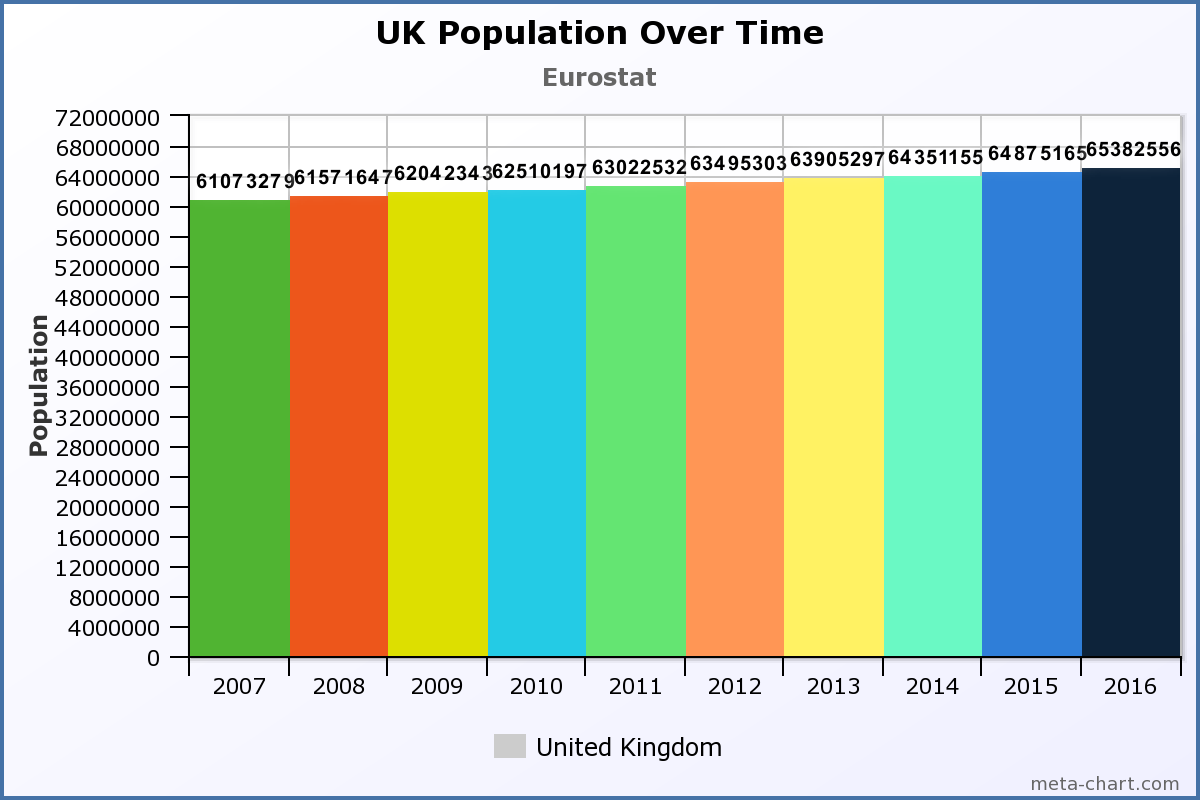
\includegraphics[width=\linewidth]{u26a2chart.png}
\begin{center}
\begin{tabular}{ |c|c|c|c|c|c|c|c|c|c| } 
	61073279,& 61571647,& 62042343,& 62510197,& 63022532, \\
	63495303,& 63905297,& 64351155,& 64875165,& 65382556  
\end{tabular}
\end{center}

As you can see, the bars are all very close, but this is due to the fact that they are all large numbers and that they are all at this range quite close. I will no generate the mean, median and mode of the information. 
\subsection{Averages}
\subsubsection{mean}
The mean is the average that most people will think of when you say average and that is because of the fact that this is the one where you add together all of the information and then divide it by the number of items in that you added. For my data set it would go like so:
\[
	1073279	+61571647	+62042343	+62510197	+63022532	+63495303	+63905297	+64351155	\\ 
\]
\[
	+64875165	+65382556
\]
\[
	/ 10
\]
\[
=	\frac{286114737}{5} 
\]
\subsubsection{median}
The median is the item that's in the middle of the numbers when the numbers are arranged in numerical order. This is useful as it completely ignore the size of the numbers that may throw some other calculations off. For this data set the median would be as follows:
\[
	61073279,	61571647,	62042343,	62510197,	63022532,
\]
\[
	63495303,	63905297,	64351155,	64875165,	65382556
\]
As you can see, in this section there is no middle value as there is an even number of terms, due to this I will select the lower of the two arbitrarily and so the answer is $ 63022532$. 
\subsubsection{mode}
The mode is the number in the series that appears the most frequently, this is used for to know what the single most popular value is. Due to the fact that the numbers in this series are all different, there is no mode and as such there is no answer to this.  
\subsection{Statistics}
In this section I will go through the Interquartile ranges, the variance and the standard deviation of the set. 
\subsubsection{interquartile ranges}
The interquartile range is defined as the range between the 3/4 and the 1/4 vales when the totals are accumulated together. Here is what they are when they are calculated:
\[
Lower quartile (xL): 61924669
\]
\[
Upper quartile (xU): 64482157.5
\]
\[
	Interquartile range (xU-xL): 1693669.75  
\]
\subsubsection{variation}
The variation is a measure of how the number are sized to each other and the values that they have the variance of my data set is as follows:
\[
	Variance: 819103702461.5
\]
\subsubsection{Standard deviation}
The standard deviation is the just the root of the variance and so its value is:
\[
	Standard Deviation: 905043.48098
\]
\subsection{Conclusion}
In conclusion you can see that I have mostly proven the hypothesis that I started out to prove. I say mostly due to the fact that most countries in the EU followed the hypothesis, however these were a few places that did not follow along with this and as such their populating went down at some point in the past 10 years. One main example is Germany and although the data is not shown the population did go down in 2010 but has been climbing since then. In addition to this there were also some places that had a declining population in the EU and as such they really do not fit my hypothesis.   
\subsection{validity}
With the results that I have collected I can say that the data derived is valid due to the fact that the information that I have derived is the same as data that other people have also collected so I can say with certainty that it is valid. Overall I think that due to this there were no errors in my data or my processing of the data so it is all good. 
\subsection{reflect}
Overall I will say that this is a success due to the fact that the data I collected was all correct and the results seemed to match those that other people had found as well. In addition to this, it matched the hypothesis that I set out to prove in the beginning which is a bonus and the correlation about this were strongly in my favour as well.  

In addition to just having the hypothesis proved, the hypothesis was true in all of the years that this was tested for which manes that I was originally very correct.  
\subsection{Theories}
In this section I will go through why I think that I got the result that I did. The main reason that I believe I got the result that I did is because the standards in the UK in general have been increasing over the years mainly in terms of healthcare but also in general with the accommodation and care of older people. The NHS would be in my opinion the main factor to this due to the fact that they offer free healthcare and this has been running for for a while and so it would have had in increasing effect during the years that I have measured in this test. In addition to this there has also been improvements in the way of life and the way that people live and now work so there has been an improvement to health and safety and to on. Due to these particular features and to few more that I have not mentioned here are the reasons that I think that the population has increased over time. Because the less people that die, the more of the population that there will be in an increasing fashion like this. 
\subsection{What if}
In this section I will go through a few 'what if' statements about the hypothesis and the result that I found from it. The first one that I will go through is what if the population of the UK would carry on to increase in the manner that it has been doing so according to the results that I have found. From the results that I have, the population at has been increasing at a rate of 397,391 new people per year, if this was to carry on then the populating would increase by one million every 3 years. If this where to carry on at this rate then the UK would be able to carry on for quite a while but after a certain point the populating would be far to large for there to be suitable housing and so on for the residents and so there would be a point where the population could not increase and this would be quite bad. 
\section{Recursion}
For this section I will go through and explaining how the binary search algorithm works and it fits in with the idea of recursion. Below you will see a basic format for the algorithm written in pseudo code:

\begin{verbatim}
for every item in the data set, read it into an array. 
if the array is not sorted then sort it
start:
go to the middle of the array 
is the current item what you are looking for?
....no: is the current item less then the item you are looking for?
........yes: remove all items in the array that are lower and return to start.
........no: remove all items in the array that are greater and return to start.
....yes: you are done as you  have found the item you are looking for, end the program. 
\end{verbatim}
As you can see here there are not many stages that are needed for the search algorithm and it is very simple to do. Due to this, the whole part of the program after start: goto will be run over and over again and this will lead to the item that you wand being found. I will now go through the algorithm step by step so that you know why each part is done like it is. 

\begin{verbatim}
for every item in the data set, read it into an array. 
\end{verbatim}
This line will read all of the information that you need into the program so that you can actually modify it and run the search. 

\begin{verbatim}
if the array is not sorted then sort it
\end{verbatim}
This line will sort the data in the array so that it is in an order that can be compared easily, like a cost or number. This will mean that later when you test if the data is greater or lower, you will know that you are removing only data that will not be correct. 

\begin{verbatim}
start:
\end{verbatim}
This line just marks this section in the code with a name so that I cat return to it later in the program. 

\begin{verbatim}
go to the middle of the array 
\end{verbatim}
This line will set the location of the program to look at the middle of the array of numbers, if the length of the array is odd then the program should just go to either one of the middle values as it does not really matter. 

\begin{verbatim}
is the current item what you are looking for?
\end{verbatim}
This will check if the item in the array that you are currently looking at in the program is actually the one that you want. This well then lead off to two conditions depending on if you have found the value that you are looking for or not. If you have found the item that you are looking for then you are done, but otherwise the program carries on. 

\begin{verbatim}
....no: is the current item less then the item you are looking for?
\end{verbatim}
This line will run if the item that the program is on is not the value that you want, that is what the no: part means. Now this is where the clever part of the algorithm starts. If the value of the item that you want is lower then where you are at the moment then you can remove all of the items that are greater than the current item as it is less then this one so it is not higher. This is why the array was sorted to start off with as now you can just remove the half of the array that is higher, and just like that you have halved the values to search. 

\begin{verbatim}
........yes: remove all items in the array that are lower and return to start.
\end{verbatim}
If the item that you are are on is lower than what you want then you can remove all of the items that are lower and this is what this section does. After you have removed the values then you can return to the start: marker of the program and recur it again. 

\begin{verbatim}
........no: remove all items in the array that are greater and return to start.
\end{verbatim}
If the item that you are are on is greater than what you want then you can remove all of the items that are greater and this is what this section does. After you have removed the values then you can return to the start: marker of the program and recur it again. 

\begin{verbatim}
....yes: you are done as you  have found the item you are looking for, end the program. 
\end{verbatim}
If the value that you have at the middle of the selection is the number that you are looking for then you have found it and can see what information it has that you need. Now you just get that information and save it and end the program and you are done. This is the terminal condition. 

\section{Use of Number Systems}
In this section I will go through how binary, octal and hexadecimal are used and are applied in areas of computing with how they are used and how they work. For this I will be showing how binary is used with ASCII, how hexadecimal is used with MIME and how Octal is used with Unix file permissions. 
\subsection{binary - ASCII}
One way that binary is used in computer science is in the use of ASCII. ASCII stands for the American Standard Code for Information Interchange and this is the standard that is used for how the standard set of English characters and numbers are encoded in binary on the computer and how it deals with them. With ASCII the letter "a" for example will have a value inside the computer of 1100001. So whenever the computer does anything with the letter a it will use this value of 1100001 internally. Now a cl;aver part of this is that "b" is 1100010, one more than "a" but the right most digits correlate to the numbers as 1 is 1 and 10 is 2. So for example if you had "s" the 19th letter in the alphabet then its ASCII value would be 1110011, and 19 in binary is 10011. This ASCII also extends to capital letters in a similar fashion as well, just with a different prefix and there is also all of the things that you can type on a English keyboard.  
\subsection{Hexadecimal - MIME}
To start off with, mime is a mechanism that enables the transmission of information in email format between computers that may not have the same language. Due to the fact that the whole point is that the computers have different languages, the 8 bits that where used in the previous example will not be enough and as such we need to use 2 Hexadecimal bits, in addition to this it also uses formatting to ensure that all messages fit a certain line length so that it is compatible and so on. This as you can see will use hexadecimal characters to represent the information and this is how they are used in computing. So, for example, a value of 12 will be "=0C". 
\subsection{Octal - Unix file permissions}
A way that octal is used in computing is in the UNIX and UNIX-like operating systems for setting file permissions for the users of the system. The way that the file permissions are handled in UNIX is that the file has meta data set aside for it that will store this information and there are 9 main bits for the file access permissions and a few more for the file type. The 9 main bits are separated into 3 sections that represent the access that the owner, group and anyone else has for the file. These 3 bits then represent the ability that they have to read, write and execute the file. So the bits are arranged like so
\begin{verbatim}
rwxrwxrwx
\end{verbatim}
As you can see, there are the 3 groups there and the (r)ead, (w)rite and e(x)ecute that the 3 groups have. Now the octal comes in when you want to change the value of these bits and the way that you do this is through the use of the chmod command. You give the chmod command the file that you want to edit and then you give it 3 octal numbers. The 3 octal numbers are then converted to binary and this then lines up with bits in the file and where there is a one that will be active. Lets say that you have a file called .xinitrc that you wanted to change the permissions of and you ran the command chmod .xinitrc 752, lets see what would happen:
\[
	7_{10} = 111_{2} \quad \& \quad 5_{10} = 101_{2} \quad \& \quad 2_{10} = 010_{2}
\]
\[
	\frac{\downarrow111101010\downarrow}{\mbox{rwxrwxrwx}} \Rightarrow \mbox{rwxr-x-w-}
\]
And now the permissions are changed using just octal numbers. This process is called masking. 
\section{Network Planning}
In this section I will go through and design 3 subnets for 3 different networks each of a different size.
\subsection{1000 hosts}
When designing a subnet you will need to find the power of 2 that is as low as possible while being higher than the target number of hosts. In this case the number is 1000, and the power of 2 that satisfies that requirement is $2^{10}$ as that is 1024. Now that I have this number I will need to then take a string of 32 ones and make, in this case the 10 rightmost ones 0's this is also known as /22 as the first 22 digits are 1's. This will mean that I now have the following:
\[
	11111111111111111111111111111111 \rightarrow 11111111111111111111110000000000
\]
Now I need to separate that number into four groups of 8 bits like so and then convert those 8 bet numbers into decimal to get the subnet mask and address:
\[
	\frac{\downarrow11111111\quad11111111\quad11111100\quad00000000\downarrow}{255 \qquad \qquad 255 \qquad \qquad 252 \qquad \qquad 000} \Rightarrow 255.255.252.0
\]
Now I have the subnet mask 255.255.252.0. And in this case this would be the most efficient and justified method for this network due to the fact that it allows for all of the devices that need to connect to the network to connect while taking up as few of the bits for the subnetting as possible so that more of these networks will be able to be up at a time. 
Another thing to note is that the network id would be 192.168.0.0. In addition to this, the broadcast would be 192.168.3.255 as that is the highest ip that is available on this network. This would mean that the any host on the network would get an ip address between these two and so there would be 1022 possible addresses for the hosts. 
\subsection{200 hosts}
with this I will do the same process but with the number 200 this time. 
	
The lowest number that satisfies what I need is $2^{8}$ as this number is 256, this is known as /24 as the first 24 bits are on. Now I will have the binary number as follows:
\[
	11111111111111111111111111111111 \rightarrow 11111111111111111111111100000000
\]
This then goes to:
\[
	\frac{\downarrow11111111\quad11111111\quad11111111\quad00000000\downarrow}{255 \qquad \qquad 255 \qquad \qquad 255 \qquad \qquad 000} \Rightarrow 255.255.255.0
\]
And so the address is 255.255.255.0. And as before this is efficient for the same reason. 
The network ID would be 192.168.0.0, the broadcast would be 192.168.0.255, this would leave 254 ip addresses between these numbers for the hosts. 
\subsection{30 hosts}
with 30 hosts the best number would be $2^{5}$ and that is 32 as that fits in all the hosts and this is /27. This would lead to the binary of this:
\[
	11111111111111111111111111111111 \rightarrow 11111111111111111111111111100000
\]
\[
	\frac{\downarrow 11111111 \quad 11111111 \quad 11111111 \quad 11100000 \downarrow}{255 \qquad \qquad 255 \qquad \qquad 255 \qquad \qquad 224} \Rightarrow 255.255.255.224
\]
And to the address is 255.255.255.224, the ID is 192.168.0.0, the broadcast is 192.168.0.32, this would leave the perfect 30 places for the hosts on the network between these values. If this network was to ever expand then they would need to use one more bit as a 0 in the mask. 
\subsection{ipv4 vs ipv6}
ipv4 and ipv6 are both ways to identify computers on a network and how they should be accessed and sent information. ipv6 is the upgraded version of the common and thoroughly used ipv4. Before I can explain the differences you need to know how they work and what they do. So, an ipv4 address will look like this: "192.168.0.1" as you can see, this is a collection of four numbers that can each go up to a total of 255 and they are all separated by a dot. This would mean that there would be a maximum of 255*255*255*255 different numbers that could happen and that is a value of 4,228,250,625. Now an ipv6 address looks like this: "2001:db8:85a3:8d3:1319:8a2e:370:7348" as you can see, this is a collection of 8 sections of 4 hexadecimal numbers each separated by a colon. Due to the fact that each block is four hexadecimal numbers the different number of possibilities are 65536, this would then go to $65526^{8}$ different possibilities and that is a huge 340282366920938463463374607431768211456. And here is the main reason that ipv6 exists, just the amount of addresses that it provides is so high. And even though the ipv4 number was big we have used all of those and so we needed to expand. 
\subsection{Network classes}
When you are talking about networks, there are a few different classes for networks that are intended for different types of networks. The types of networks are called class A, B and C. These are distinguished by the subnet mark that they use.  \\
\begin{matrix}
	Class  & First ID  &  Last ID \\
	Class A &	1.0.0.0	    & 126.0.0.0 \\
	Class B &	128.0.0.0 &	191.255.0.0 \\
	Class C	 & 192.0.0.0 &	223.255.255.0
\end{matrix}
\\
From this you can see that the Last ID will be the same as the subnet mask for the network and then the first ID will be the first ip address that will be available. As you can see, the class A networks will have the ability to have many, many devices connected at the same time, but not many of then can be connected. Due to this there networks are used by ISP's because that is what they need. On the other end of the scale you have the Class C networks and these cannot have too many devices connected to them but there can be a lot of them. Due to this this would be suited to the home owners that the ISP will serve, and that is what happens. All the classes in-between are used by companies of different sizes and so on.  
\subsection{Classless Inter Domain Routing (CIDR) }
The final part on this networking section is the CIDR, this stand for Classless Inter Domain Routing and is a way of allow there to be more ip addresser allocated to devices while still keeping the existing infrastructure in place. If you look at how subnetting allows there to be more networks connected together which in turn adds in more ip addresses to be able to be used in there own networks. This is how supernetting or CIDR works but instead you perform the action on the subnets which in turn performs the process on the ip addresses. Using this as you can see, you can get many more subnets and in turn many more ip addresses and hosts connected to the network. 
\section{conclusion}
In conclusion you can see that I have managed to show you that I understand the maths and behind all the criteria in this assignment. 

\end{document}
